% Author: Izaak Neutelings (July 2018)
\documentclass[border=3pt,tikz]{standalone}
\usepackage{tikz}
\usepackage{physics}
\tikzset{>=latex} % for LaTeX arrow head
\usetikzlibrary{angles,quotes} % for pic (angle labels)
\usepackage{xcolor}
\colorlet{pinkskin}{pink!25}
\colorlet{brownskin}{pink!5!brown!45}
\colorlet{myred}{red!90!black}
\colorlet{myblue}{blue!90!black}
\colorlet{mypurple}{blue!50!red!80!black!80}
\colorlet{Bcol}{violet!90}
\colorlet{BFcol}{red!60!black}
\colorlet{veccol}{green!45!black}
\colorlet{Icol}{blue!70!black}
\colorlet{mucol}{red!90!black}
\tikzstyle{BField}=[->,line width=2,Bcol]
\tikzstyle{current}=[->,Icol] %thick,
\tikzstyle{force}=[->,line width=2,BFcol]
\tikzstyle{vector}=[->,line width=2,veccol]
\tikzstyle{thick vector}=[->,line width=2,veccol]
\tikzstyle{mu vector}=[->,line width=2,mucol]
\tikzstyle{velocity}=[->,line width=2,veccol]
\tikzstyle{charge+}=[very thin,draw=black,top color=red!50,bottom color=red!90!black,shading angle=20,circle,inner sep=0.5]


\begin{document}
\Large
% RIGHT HAND RULE xyz
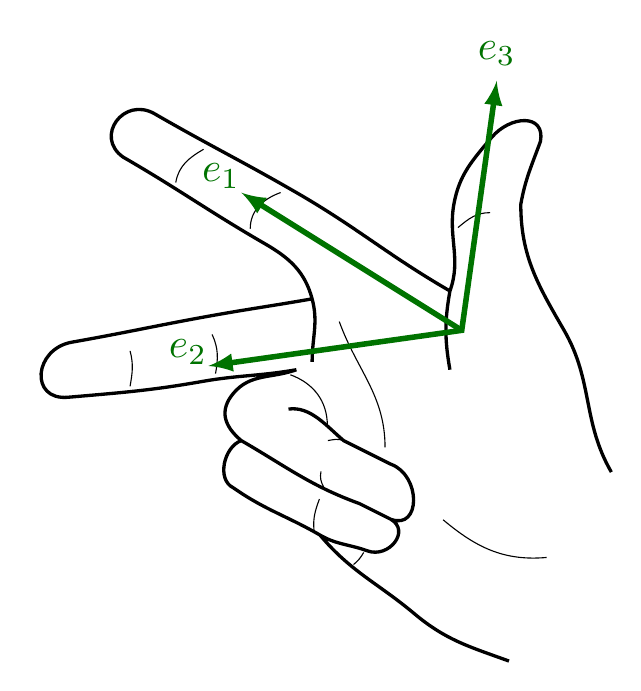
\begin{tikzpicture}
  \coordinate (O) at (1.0,0.7); % ORIGIN
  \coordinate (WT) at ( 2.9,-1.1); % WRIST TOP
  \coordinate (T1) at ( 2.3, 0.7); % THUMB
  \coordinate (T2) at ( 1.75, 2.3);
  \coordinate (T3) at ( 2.0, 3.1);
  \coordinate (T4) at (1.38, 3.15);
  \coordinate (T5) at ( 0.9, 2.3);
  \coordinate (T6) at ( 0.85, 1.2);
  \coordinate (T7) at ( 0.85, 0.2);
  \coordinate (I1) at (-1.1, 2.45); % INDEX
  \coordinate (I2) at (-2.9, 3.45);
  \coordinate (I3) at (-3.3, 2.9);
  \coordinate (I4) at (-1.5, 1.8);
  \coordinate (I5) at (-0.9, 1.1);
  \coordinate (I6) at (-0.9, 0.3);
  \coordinate (M1) at (-2.1, 0.9); % MIDDLE
  \coordinate (M2) at (-3.95,0.55);
  \coordinate (M3) at (-4.0,-0.15);
  \coordinate (M4) at (-2.3, 0.05);
  \coordinate (M5) at (-1.1, 0.20);
  \coordinate (R1) at (-1.9,-0.1); % RING
  \coordinate (R2) at (-1.8,-0.7);
  \coordinate (R3) at (-0.3,-1.5);
  \coordinate (R4) at ( 0.1,-1.7);
  \coordinate (R5) at ( 0.1,-1.0);
  \coordinate (R6) at (-0.5,-0.7);
  \coordinate (R7) at (-1.2,-0.3);
  \coordinate (P1) at (-1.9,-1.3); % PINKY
  \coordinate (P2) at (-0.8,-1.9);
  \coordinate (P3) at (-0.2,-2.1);
  \coordinate (P4) at (-0.05,-1.65);
  \coordinate (W1) at ( 0.4,-2.9); % WRIST BOTTOM
  \coordinate (W2) at ( 1.6,-3.5);
  
  % HAND
  %\fill[pinkskin] (WT) -- (T6) -- (I5) -- (M5) -- (R2) -- (P2) -- (W2) to[out=25,in=-90] cycle;
  \draw[very thick]
    (WT) to[out=120,in=-60] % THUMB
    (T1) to[out=120,in=-90]
    (T2) to[out=80,in=-110]
    (T3) to[out=80,in=50,looseness=1.5] % tip
    (T4) to[out=-130,in=80]
    (T5) to[out=-100,in=70]
    (T6) to[out=-100,in=100]
    (T7)
    (T6) to[out=150,in=-30] % INDEX
    (I1) to[out=150,in=-30]
    (I2) to[out=150,in=145,looseness=1.7] % tip
    (I3) to[out=-30,in=150]
    (I4) to[out=-30,in=105]
    (I5) to[out=-75,in=90]
    (I6)
    (I5) to[out=-170,in=10] % MIDDLE
    (M1) to[out=-170,in=10]
    (M2) to[out=-170,in=-175,looseness=1.8] % tip
    (M3) to[out=5,in=-170]
    (M4) to[out=10,in=-170] % bottom knuckle
    (M5)
    (M5) to[out=-160,in=50] % RING
    (R1) to[out=-130,in=140,looseness=1.2]
    (R2) to[out=-30,in=160]
    (R3) --
    (R4) to[out=-20,in=-20,looseness=1.5] % tip
    (R5) --
    (R6) to[out=140,in=8,looseness=0.9]
    (R7)
    (R2) to[out=-160,in=155] % PINKY
    (P1) to[out=-35,in=150]
    (P2) to[out=-30,in=160]
    (P3) to[out=-20,in=-30,looseness=1.5] % tip
    %(P4) --
    (R4)
    (P2) to[out=-50,in=140] % WRIST
    (W1) to[out=-40,in=160]
    (W2);
  
  % FOLDS
  \draw (T5)++(-80:0.3) to[out=40,in=180]++ (25:0.45); % THUMB
  \draw (I1)++(180:0.2) to[out=-160,in=90]++ (-130:0.6); % INDEX
  \draw (I1)++(155:1.3) to[out=-150,in=80]++ (-130:0.55);
  \draw (M4)++(30:0.2) to[out=80,in=-65]++ (95:0.5); % MIDDLE FINGER
  \draw (M3)++(10:0.8) to[out=80,in=-75]++ (90:0.45);
  \draw (M5)++(-140:0.1) to[out=-20,in=90]++ (-54:0.8); % RING
  \draw (R6) to[out=160,in=10]++ (180:0.2);
  \draw (R3)++(155:0.5) to[out=120,in=-100]++ (100:0.2);
  \draw (P2)++(140:0.1) to[out=95,in=-110]++ (80:0.4); % PINKY
  %\draw (P1)++( 10:0.04) to[out=95,in=-130]++ (70:0.4);
  \draw (I5)++(-40:0.45) to[out=-70,in=90]++ (-70:1.7);    % PALM
  \draw (P3)++(-155:0.05) to[out=-120,in=40]++ (-130:0.2); % PALM
  \draw (W2)++(70:1.4) to[out=-175,in=-40]++ (160:1.4); % PALM
  
  % VECTORS
  \def\R{0.32}
  \draw[thick vector]
    (O) --++ (148:3.3) coordinate (X) node[above=6,left=-6,scale=1.5] {$e_1$};
  \draw[thick vector,<->]
    (O) ++ (-172:3.25) coordinate (Y) node[above=5,left=-6,scale=1.5] {$e_2$} --
    (O) --++ (82:3.2) node[above=-1,scale=1.5] {$e_3$};
  
\end{tikzpicture}
\end{document}